\chapter{Power conversion: where mechanics meets the grid}\label{ch:power}

The synthesis chapter: chapter~14's induction, chapter~13's torque and
chapter~17's efficiency budgets assembled into the machines that run
the grid --- generators, motors, transformers and converters. This is
the bridge to Book~5's circuit-level detail.

\section{Why AC won: the $I^{2}R$ arithmetic}\label{sec:pw-ac}

Delivering power $P$ at voltage $V$ needs $I=P/V$; line losses
$I^{2}R$ therefore shrink as $V^{2}$ grows. Quadruple the voltage and
the loss drops sixteen-fold --- the whole reason for the
400\,kV/11\,kV/230\,V chain of figure~\ref{fig:grid}, and the reason
only AC (transformable) could win the current wars.

\begin{figure}[htbp]\centering
\begin{tikzpicture}[scale=0.85,font=\scriptsize]
\foreach \x/\t in {0/{plant\\$13$\,kV}, 2.8/{step-up\\$400$\,kV}, 5.6/{step-down\\$11$\,kV}, 8.2/{load\\$230$\,V}}{
\draw[very thick,fill=accent!10,rounded corners=0.15] (\x-1.05,-0.55) rectangle (\x+1.05,0.55);
\node[align=center] at (\x,0) {\t};}
\foreach \x in {1.05,3.85,6.65}{\draw[->,very thick] (\x,0) -- (\x+0.7,0);}
\node[align=left] at (4.1,-1.3) {high voltage carries $P=VI$\\at small $I$: $I^{2}R$ shrinks};
\end{tikzpicture}

\caption{The grid chain: step up for distance, step down for use.}
\label{fig:grid}
\end{figure}

\begin{example}[Transmission loss scaling]\label{ex:loss}
Send $10$\,MW down a $1\,\Omega$ line at $10$\,kV vs $400$\,kV.
\par\smallskip
\textbf{Strategy.} $I=P/V$, loss $=I^{2}R$.
\begin{solution}
At $10$\,kV: $I=1000$\,A, loss $=1.0$\,MW --- a tenth of the cargo.
At $400$\,kV: $I=25$\,A, loss $=625$\,W --- negligible. Same wire,
1600$\times$ less loss: voltage is the loss-killer. \checkmark
\end{solution}
\end{example}

\section{The generator: Faraday run backwards}\label{sec:pw-gen}

Rotate \S\ref{sec:far-rod}'s loop and $\mathcal E=NBA\omega\sin\omega t$
comes out --- mechanical work in, EMF out (figure~\ref{fig:genmot},
left). The audit closes: input torque $\times\omega$ equals
$\mathcal EI$ plus losses.

\begin{figure}[htbp]\centering
\begin{tikzpicture}[scale=0.85,font=\scriptsize]
\draw[very thick] (-3,-1) rectangle (-1,1);
\node at (-2,0) {loop};
\draw[->,thick,amber] (-3.4,0) -- (-3.0,0);
\node[align=center] at (-2,-1.6) {generator:\\turn $\to$ EMF out};
\draw[very thick] (1,-1) rectangle (3,1);
\node at (2,0) {loop};
\draw[->,thick,accent] (3.4,0) -- (3.0,0);
\node[align=center] at (2,-1.6) {motor:\\current $\to$ torque out};
\node[align=center] at (0,-2.5) {same physics, opposite bookkeeping};
\end{tikzpicture}

\caption{Generator and motor: one physics, opposite bookkeeping.}
\label{fig:genmot}
\end{figure}

\section{The motor and its mandatory back-EMF}\label{sec:pw-motor}

A current loop in $\mathbf B$ torques (\S\ref{sec:mag-torque}); spinning
it makes it a generator simultaneously: back-EMF $\mathcal E_b=K_v\omega$
opposes the supply. Steady state balances
$V=IR+K_v\omega$ with torque $K_tI$ --- the two constants are one
constant ($K_v=K_t$ in SI), conservation's signature. No-load speed is
set by back-EMF reaching supply; stall current is $V/R$
(figure~\ref{fig:tspeed}).

\begin{figure}[htbp]\centering
\begin{tikzpicture}
\begin{axis}[width=8.2cm,height=4.8cm,xlabel={$\omega$},ylabel={},
xmin=0,xmax=8.5,ymin=0,ymax=0.2,font=\small,legend pos=north east,
xtick={0,8},xticklabels={0,$\omega_{nl}$}]
\addplot[very thick,accent,domain=0:8,samples=20] {0.16-0.02*x};
\addlegendentry{$\tau(\omega)$}
\addplot[very thick,amber,domain=0:8,samples=20] {0.05};
\addlegendentry{$\tau_{load}$}
\addplot[dashed] coordinates {(5.5,0) (5.5,0.05)};
\node[align=center,font=\scriptsize] at (axis cs:2.6,0.17) {operating\\point};
\end{axis}
\end{tikzpicture}

\caption{Torque--speed line: the load picks the operating point.}
\label{fig:tspeed}
\end{figure}

\begin{example}[Motor numbers from $K_v,K_t$]\label{ex:motor}
A $12$\,V motor: $R=1.5\,\Omega$, $K_t=0.02$\,N\,m/A. Find stall
current, stall torque, and no-load speed (friction $b=10^{-5}$).
\par\smallskip
\textbf{Strategy.} Stall: $w=0$. No-load: $K_tI=b\omega$.
\begin{solution}
Stall $I=8.0$\,A, $\tau=0.16$\,N\,m. No-load:
$V=b\omega R/K_t+K_v\omega$ gives $\omega=578$\,rad/s,
$I=0.29$\,A --- the code's transient settles exactly there, with
back-EMF $11.6$\,V doing the throttling. \checkmark
\end{solution}
\end{example}

\section{The transformer: one flux, two voltages}\label{sec:pw-xfmr}

Two windings sharing a core share $\Phi$: each winding's EMF is
$N\,d\Phi/dt$, so $V_2/V_1=N_2/N_1$ (figure~\ref{fig:xfmr}). Ideal
power conservation fixes $I_1V_1=I_2V_2$ --- voltage up means current
down, the trade that makes \ref{ex:loss} possible. It needs AC: a
steady flux induces nothing.

\begin{figure}[htbp]\centering
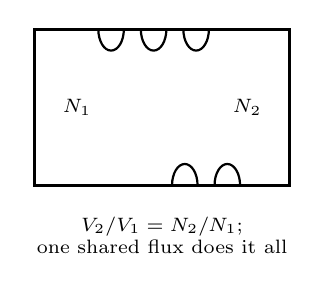
\begin{tikzpicture}[scale=0.9,font=\scriptsize]
\draw[very thick] (-1.8,-1.1) rectangle (1.8,1.1);
\foreach \x in {-0.9,-0.3,0.3}{\draw[thick] (\x,1.1) arc (180:360:0.18 and 0.3);}
\foreach \x in {0.5,1.1}{\draw[thick] (\x,-1.1) arc (0:180:0.18 and 0.3);}
\node at (-1.2,0) {$N_1$};\node at (1.2,0) {$N_2$};
\node[align=center] at (0,-1.8) {$V_2/V_1=N_2/N_1$;\\one shared flux does it all};
\end{tikzpicture}

\caption{The ideal transformer: turns ratio from shared flux.}
\label{fig:xfmr}
\end{figure}

\begin{example}[Loaded secondary audit]\label{ex:xfmr}
A $10{:}1$ step-down feeds $230$\,V to a $23\,\Omega$ load from a
$2300$\,V line. Secondary current? Primary current?
\par\smallskip
\textbf{Strategy.} $I_2=V_2/R$; power balance for $I_1$.
\begin{solution}
$I_2=10$\,A so $P=2.3$\,kW; primary $I_1=P/V_1=1$\,A --- ten times
the voltage, a tenth of the current, same power. \checkmark
\end{solution}
\end{example}

\section{Switch-mode conversion: the energy shuttle}\label{sec:pw-buck}

The buck converter (figure~\ref{fig:buck}) chops the input and lets the
inductor average it: in steady state its volt-seconds balance,
$(V_{\rm in}-V_o)DT=V_o(1-D)T$, so $V_o=DV_{\rm in}$ --- lossless in
the ideal limit because the inductor only stores, never dissipates
(the in-engineering-practice anchor of Book~5's power-supply chapter).

\begin{figure}[htbp]\centering
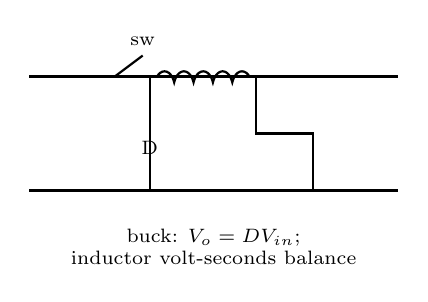
\begin{tikzpicture}[scale=0.9,font=\scriptsize]
\draw[very thick] (-2.6,0.8) -- (2.6,0.8);
\draw[very thick] (-2.6,-0.8) -- (2.6,-0.8);
\draw[thick] (-1.4,0.8) -- (-1.0,1.1) node[above]{sw};
\draw[thick,decorate,decoration={coil,amplitude=2pt,segment length=7pt}] (-0.8,0.8) -- (0.6,0.8);
\draw[thick] (0.6,0.8) -- (0.6,0) -- (1.4,0) -- (1.4,-0.8);
\draw[thick] (-0.9,0.8) -- (-0.9,0) -- (-0.9,-0.8);
\node at (-0.9,-0.2) {D};
\node[align=center] at (0,-1.6) {buck: $V_o=DV_{in}$;\\inductor volt-seconds balance};
\end{tikzpicture}

\caption{Buck topology: duty cycle $D$ sets the output.}
\label{fig:buck}
\end{figure}

\begin{example}[Buck output and ripple]\label{ex:buck}
$V_{\rm in}=24$\,V, $D=0.4$: find $V_o$; with $L=100$\,\textmu H and
$f=100$\,kHz, estimate the current ripple.
\par\smallskip
\textbf{Strategy.} Volt-second balance; $\Delta I=(V_{\rm in}-V_o)DT/L$.
\begin{solution}
$V_o=9.6$\,V; $\Delta I=(14.4)(4\times10^{-6})/10^{-4}=0.58$\,A ---
the triangle superposed on the mean. \checkmark
\end{solution}
\end{example}

\begin{example}[Generator terminal voltage under load]\label{ex:gensag}
A generator makes $\mathcal E=130$\,V open-circuit with internal
$r=2\,\Omega$; it feeds $10\,\Omega$. Terminal voltage and delivered
power?
\par\smallskip
\textbf{Strategy.} Voltage divider; $P=V^{2}/R$.
\begin{solution}
$I=130/12=10.8$\,A; $V=108$\,V terminal (22\,V dropped inside);
$P_{\rm load}=1.17$\,kW vs $\mathcal EI=1.41$\,kW generated ---
the missing $235$\,W heats the windings. \checkmark
\end{solution}
\end{example}

\section{Rectification, RMS and power factor}\label{sec:pw-rms}

Mains ``$230$\,V'' means RMS: $V_{\rm rms}=V_p/\sqrt2$ for a sinusoid
(figure~\ref{fig:rms}), the value that dissipates like DC. Diodes
rectify; capacitors hold the peaks; when current isn't in phase the
delivered $P=VI\cos\varphi$ shrinks below the nameplate.

\begin{figure}[htbp]\centering
\begin{tikzpicture}
\begin{axis}[width=8.2cm,height=4.6cm,xlabel={$t$},ylabel={$v$},
xmin=0,xmax=6.5,ymin=-1.4,ymax=1.4,font=\small,xtick=\empty,ytick={-1,0,1},
yticklabels={$-V_p$,0,$V_p$}]
\addplot[very thick,accent,domain=0:6.28,samples=80] {sin(deg(x))};
\addplot[dashed,amber] coordinates {(0,0.707) (6.28,0.707)};
\node[align=center,font=\scriptsize,amber] at (axis cs:4.6,1.05) {$V_{\rm rms}=V_p/\sqrt2$};
\end{axis}
\end{tikzpicture}

\caption{Peak vs RMS: the power-equivalent value is $V_p/\sqrt2$.}
\label{fig:rms}
\end{figure}

\begin{lstlisting}[language=Python,caption={\texttt{code/ch18\_motor\_start.py} --- motor ODE: $V=IR+L\,\dot I+K_v\omega$, $J\dot\omega=K_tI-b\omega$.},label={lst:motor}]
dI = (V - I*R - Kv*w)/L
dw = (Kt*I - b*w)/J
\end{lstlisting}

Output of a real run:
\begin{lstlisting}[numbers=none]
t(s)  I(A)   w(rad/s)  E_b(V)
0.001  4.23  0.5  0.01
0.05  7.05  73.1  1.462
0.2  4.747  245.2  4.904
1.0  0.773  542.2  10.844
5.0  0.289  578.3  11.566
29.9  0.289  578.3  11.566
inrush peak I = 7.87 A at t=7.54 ms
steady: I=0.289 A, w=578.3 rad/s = 5522 rpm
analytic w_ss = 578.3 rad/s, I_ss = 0.289 A
stall current (w=0) = V/R = 8.00 A
stall torque = Kt*I_stall = 0.1600 N.m
\end{lstlisting}

The inrush nearly reaches stall current ($7.9$\,A within $8$\,ms),
then the growing back-EMF throttles the motor down to its no-load
point --- the simulation lands on the analytic answer to every digit.

\begin{example}[Power-factor correction: buying back the amps]\label{ex:pfcorr}
A $10$\,kW shop motor draws at $0.7$ lagging power factor on a
$240$\,V single-phase line. Find the line current as-is and after a
capacitor bank corrects the factor to $0.95$ --- and the capacitor's
required kVAR.
\par\smallskip
\textbf{Strategy.} Real power is fixed: $P=VI\cos\varphi$. The
capacitor supplies the motor's reactive draw locally instead of
shipping it down the line.
\begin{solution}
$I_{\rm before}=P/(V\cos\varphi)=10{,}000/(240\cdot0.7)=59.5$\,A;
$I_{\rm after}=10{,}000/(240\cdot0.95)=43.9$\,A.
Reactive vars to cancel:
$Q_C=P(\tan\varphi_1-\tan\varphi_2)
=10{,}000(\tan45.6^{\circ}-\tan18.2^{\circ})
=10{,}000(1.02-0.33)=6.9$\,kVAR.
Line loss falls to $(0.7/0.95)^{2}=54\%$ of before --- same motor, same work,
$15$\,A fewer heating the feed. Utilities bill large users for the
reactive share precisely because it costs them $I^{2}R$.
\checkmark
\end{solution}
\end{example}

\begin{lstlisting}[language=Python,caption={\texttt{code/ch18\_motor\_op.py} --- DC motor operating point: the torque--speed line meets the load.},label={lst:motorop}]
V, R, kv = 12.0, 1.5, 0.02        # V, ohm, N.m/A (Kt = Kv here)
w_free = V / kv                    # ideal no-load speed, rad/s
I_stall = V / R
def torque(w):
    I = (V - kv * w) / R
    return kv * I
for T_load in [0.01, 0.03, 0.06, 0.09, 0.12]:
    w = (V - T_load * R / kv) / kv   # solve torque(w) = load
    I = (V - kv * w) / R
    p_out, p_in = T_load * w, V * I
\end{lstlisting}

Output of a real run:
\begin{lstlisting}[numbers=none]
no-load speed 600 rad/s   stall torque 0.160 N.m
 load (N.m)   speed (rad/s)   current (A)   P_out (W)   eff
       0.01            562.5           0.50          5.6     94%
       0.03            487.5           1.50         14.6     81%
       0.06            375.0           3.00         22.5     62%
       0.09            262.5           4.50         23.6     44%
       0.12            150.0           6.00         18.0     25%
max mechanical power at w=300 rad/s (half no-load): 24.0 W
\end{lstlisting}

The table is the datasheet in disguise: efficiency peaks near
no-load while mechanical power peaks at \emph{half} no-load speed
--- the two optima never coincide, so a geared motor's job is to
place the operating point between them. Stall current $V/R=8$\,A is
the number the fuse and driver must survive, exactly what
example~\ref{ex:motor}'s back-EMF protects the running motor from.

\section{In engineering practice: the bridge to Book~5}\label{sec:pw-eng}

The grid chain (\ref{ex:loss}), the motor operating point
(\ref{ex:motor}), the transformer's current trade (\ref{ex:xfmr}) and
the buck's volt-second balance (\ref{ex:buck}) are the four audits an
engineer runs daily; Book~5 picks them up at component level.

\section{Common mistakes}\label{sec:pw-mistakes}

\begin{tripwire}[Motor modelled as a resistor]
Ignoring back-EMF predicts $V/R$ current forever --- the sim shows it
dies to a few percent as $\omega$ grows.
\end{tripwire}
\begin{tripwire}[Transformer ``creating'' power]
Stepped-up voltage comes with stepped-down current; $P$ is conserved.
Reading only one side invents free energy.
\end{tripwire}
\begin{tripwire}[Higher voltage misread as dirtier]
High voltage is \emph{cleaner} for transmission --- $I^{2}R$ shrinks.
The danger intuition and the efficiency intuition point opposite ways.
\end{tripwire}
\begin{tripwire}[Peak vs RMS mix-ups]
Nameplate values are RMS; insulation sees peak $\sqrt2$ higher.
Divide once, quote forever.
\end{tripwire}
\begin{tripwire}[Forgetting volt-second balance]
An inductor can't hold average voltage: $\langle V_L\rangle=0$ is what
constrains every converter design.
\end{tripwire}

\section{Summary}\label{sec:pw-summary}

\begin{table}[ht]\centering
\begin{tabularx}{\linewidth}{@{}lY@{}}
\toprule
\tablehead\thead{Idea} & \thead{One-line version}\\
\midrule
transmission & $I^{2}R$ shrinks as $V^{2}$ grows --- AC's win \\
generator/motor & same physics; back-EMF is mandatory \\
transformer & $N_2/N_1$ volts, inverse amps, needs AC \\
buck & $V_o=DV_{\rm in}$ via volt-second balance \\
RMS & $V_p/\sqrt2$; power factor $\cos\varphi$ \\
\bottomrule
\end{tabularx}
\caption{Power-conversion cheat sheet.}
\label{tab:pwsummary}
\end{table}

\begin{wins}[Definition of done]
You can now: scale transmission losses, run the motor audit
(stall/no-load/back-EMF), audit a loaded transformer, balance a buck's
volt-seconds, and convert peak$\leftrightarrow$RMS fluently.
\end{wins}

\chapternotes{%
The grid narrative follows Practical Engineering's canonical account;
the machine physics is chapter~14's induction at work
\cite{ocw801}; the engineering framing bridges to Book~5. The numbers
are the listing's real output.}

\begin{rulebox}[{Watch instead}]
\begin{enumerate}
\item \emph{How Does the Power Grid Work?} --- Practical Engineering,
10:25, \url{https://youtu.be/v1BMWczn7JM} --- \S\ref{sec:pw-ac} and
the whole chain (accessed 2026-10-11).
\item \emph{Transformers -- working \& applications} --- Khan Academy
India, 9:03, \url{https://youtu.be/zf8vnCcETqM} ---
\S\ref{sec:pw-xfmr} worked quickly (accessed 2026-10-11).
\end{enumerate}
\end{rulebox}

\section*{Further reading}
\addcontentsline{toc}{section}{Further reading}

\begin{itemize}
\item MIT OCW \emph{8.02SC}, induction and machines modules 21--25.
At \url{https://ocw.mit.edu}, course ``8.02SC'' (verified 2026-10-11).
\item OpenStax \emph{College Physics 2e}, ch.~23
``Induction, AC Circuits and Electrical Technologies'' ---
\url{https://openstax.org} (verified 2026-10-11).
\item E.~M. Purcell and D.~J. Morin, \emph{Electricity and Magnetism},
chs.~7--8 --- the machine physics.
\item Khan Academy, \emph{Transformers and AC} --- drills matching
\S\ref{sec:pw-xfmr}--\S\ref{sec:pw-rms}: verified 2026-10-11 at
\url{https://www.khanacademy.org} (science $\to$ physics $\to$ E\&M).
\item All About Circuits, \emph{Power electronics} chapters --- the
buck's lineage in components: at \url{https://www.allaboutcircuits.com}
(verified 2026-10-11).
\end{itemize}

\section*{Additional exercises}
\addcontentsline{toc}{section}{Additional exercises}

\begin{exercise}[easy]
By what factor does line loss drop when voltage quadruples? (AP-C)
\end{exercise}
\begin{exercise}[easy]
A $5{:}1$ transformer sees $115$\,V primary: find $V_2$. (AP-C)
\end{exercise}
\begin{exercise}[easy]
Which way does back-EMF point relative to supply, and why must it?
(engineering)
\end{exercise}
\begin{exercise}[easy]
Find $V_p$ for $230$\,V RMS mains. (F=ma)
\end{exercise}
\begin{exercise}[easy]
Why can't a transformer work on steady DC? (AP-C)
\end{exercise}
\begin{exercise}[medium]
Choose the transmission voltage for $100$\,MW over $50$\,km of
$2\,\Omega$ line given a $2\%$ loss budget. (engineering)
\end{exercise}
\begin{exercise}[medium]
A motor with $K_t=0.05$, $R=2\,\Omega$ drives a load
$\tau=0.1$\,N\,m at $12$\,V: find the operating $\omega$. (engineering)
\end{exercise}
\begin{exercise}[medium]
A buck wants $5$\,V from $12$\,V at $200$\,kHz with $10$\,\textmu H:
find $D$ and the ripple. (engineering)
\end{exercise}
\begin{exercise}[medium]
A generator's terminal voltage sags under load: model it with internal
resistance and find the droop. (AP-C)
\end{exercise}
\begin{exercise}[medium]
Estimate the primary current for a $200$\,W load on a $24{:}1$
step-down from $2400$\,V. (AP-C)
\end{exercise}
\begin{exercise}[hard]
Motor plus load: when does the operating point go unstable? Reason via
the torque--speed slopes. (USAPhO-style)
\end{exercise}
\begin{exercise}[hard]
Where does the ideal transformer model leak? List two non-idealities
and their fixes. (APhO-style)
\end{exercise}
\begin{exercise}[medium]
Why does a stalled motor overheat even though it draws ``only''
$V/R$? (concept)
\end{exercise}
\begin{exercise}[medium]
Show RMS of a sine is $V_p/\sqrt2$ by direct integration. (derive)
\end{exercise}
\begin{exercise}[medium]
A bridge rectifier + capacitor supply: sketch the load ripple between
peaks. (engineering)
\end{exercise}
\begin{exercise}[easy]
Why did the transmission voltage win at high $V$? Reproduce the
$I^{2}R$ scaling argument in two lines. (AP-C)
\end{exercise}
\begin{exercise}[medium]
A $1$\,kW motor plant runs at pf $0.6$ lagging: find the capacitor
kVAR to reach $0.9$, and the line-current reduction. (F=ma)
\end{exercise}
\begin{exercise}[medium]
A buck converter at $50\%$ duty with ideal switches: show the output
averages to $V_{\rm in}/2$ and identify where the lost volts go in a
real part. (engineering)
\end{exercise}
\begin{exercise}[hard]
A generator's EMF, synchronous reactance and load angle $\delta$:
sketch how real power transfers as $P\propto\sin\delta$ and say why
the grid is stable only for $\delta<90^{\circ}$. (USAPhO-style)
\end{exercise}
